\documentclass[14pt]{beamer}
\usepackage[utf8]{inputenc}

\mode<presentation>{ \usetheme{Madrid}

% To remove the navigation symbols from the bottom of all slides uncomment next line
\setbeamertemplate{navigation symbols}{}
\date{}
\title{}
\author{}

%to get rid of footer entirely uncomment next line
\setbeamertemplate{footline}{}
}

\usepackage{geometry}
\usepackage{multirow}
\usepackage{adjustbox}
\usepackage{multicol}
\setlength{\columnsep}{0.1cm}

\usepackage{tikz}
\usetikzlibrary{shapes, backgrounds}

\usepackage{bbding}
\usepackage{rotating}
\usepackage{xcolor}

%\usepackage{tkz-berge} %cool grid
\usepackage{pgfplots} %pics

\usepackage{graphicx} % Allows including images
\usepackage{
	booktabs
} % Allows the use of \toprule, \midrule and \bottomrule in tables
\usepackage{mathtools}

\newcommand{\DS}[1]{$\displaystyle #1$}
\newcommand{\R}{\mathbb{R}}
\newcommand{\Z}{\mathbb{Z}}
\newcommand{\N}{\mathbb{N}}
\newcommand{\e}{\varepsilon}

\newcommand{\p}{\pause}

% simple environrment for enumerate, easier to read
\setbeamertemplate{enumerate items}[default]

%%%%%%%%%%%%%%%%%%%%%%

% to use colours easily
\definecolor{verde}{rgb}{0, .8, 0}
\definecolor{rosa}{rgb}{1, 0, 1}
\definecolor{naranja}{rgb}{1, .5, 0.1}
\newcommand{\azul}[1]{{\color{blue} #1}}
\newcommand{\rojo}[1]{{\color{red} #1}}
\newcommand{\verde}[1]{{\color{verde} #1}}
\newcommand{\rosa}[1]{{\color{rosa} #1}}
\newcommand{\naranja}[1]{{\color{naranja} #1}}
\newcommand{\violeta}[1]{{\color{violet} #1}}

% box in red and blue in math and outside of math
\newcommand{\cajar}[1]{\boxed{\mbox{\rojo{ #1}}}}
\newcommand{\majar}[1]{\boxed{\rojo{ #1}}}
\newcommand{\cajab}[1]{\boxed{\mbox{\azul{ #1}}}}
\newcommand{\majab}[1]{\boxed{\azul{ #1}}}

\newcommand{\setsize}[1]{\fontsize{#1}{#1}\selectfont} %allows you to change the font size. The default size of this document is 14. To change the font size of the whole slide, place this at the beginning of the slide. To change the size of only a portion of the text to size 12, you can do the following { \setsize{12} Your text. }.

\setbeamerfont{frametitle}{size=\setsize{15}}
\setbeamerfont{block title}{size=\setsize{14}}

\newcommand{\smallerfont}{\setsize{13}} %place this at the beginning of a slide to set the font size of the entire slide to 13.

%===========================
% Preamble just for this file
%===========================

\newcommand{\arcsec}{\operatorname{arcsec}}

\setbeamertemplate{enumerate items}{(\Alph{enumi})}
%===================================================
\begin{document}
	%===================================================

\begin{frame}
	\frametitle{MAT137 Lecture 26 --- Local Extrema}

	{\bf Warmup:}

	Write down, in set-builder notation, the domain of $\tan$, the tangent function.

	\vfill
	{\bf Before next class:}
		\begin{itemize} \normalsize
			\item {\bf Watch videos  5.5, 5.6}
		\end{itemize}
\end{frame}

	%-----------------------------
	\begin{frame}
		\frametitle{Definition of local extremum}

		Find local and global extrema of the function with this graph:

		\begin{center}
			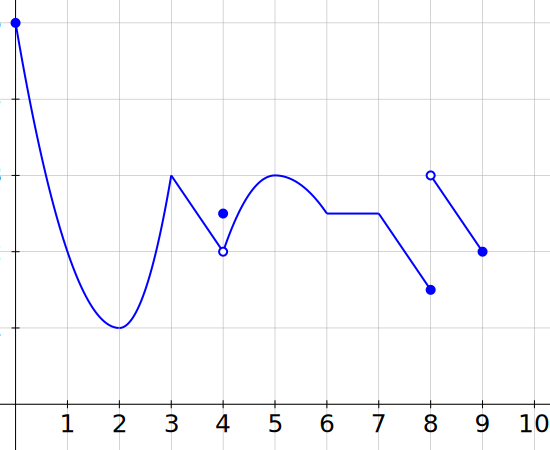
\includegraphics[scale=.42]{G13}
		\end{center}
	\end{frame}
	%-----------------------------
	\begin{frame}[t]
		\frametitle{Where is the maximum?}

		We know the following about the function $h$:
		\begin{itemize}
			\item The domain of $h$ is $\displaystyle (-4,4)$.

			\item $h$ is continuous on its domain.

			\item $h$ is differentiable on its domain, except at $0$.

			\item $h'(x) = 0 \quad \iff \quad x=-1 \mbox{ or }1$.
		\end{itemize}

		\begin{block}{What can you conclude about the maximum of $h$?}
			\pause
			\begin{enumerate}
				\item $h$ has a maximum at $x=-1$, or $1$.

				\item $h$ has a maximum at $x=-1,0,$ or $1$.

				\item $h$ has a maximum at $x=-4, -1,0, 1,$ or $4$.

				\item None of the above.
			\end{enumerate}
		\end{block}
	\end{frame}


	\begin{frame}[t]
		\frametitle{Fractional exponents}

		Let $\displaystyle  g(x) = x^{2/3} (x-1)^3. $

		\medskip
		Find local and global extrema of $g$ on $\displaystyle [-1,2]$.
	\end{frame}

	\begin{frame}[t]
		\frametitle{Trig extrema}

		Let $\displaystyle  f(x) = \frac{\sin x}{3 + \cos x}. $

		\medskip
		Find the maximum and minimum of $f$.
	\end{frame}









\begin{frame}
	\frametitle{MAT137 Lecture 27 --- Rolle's Theorem}

	{\bf Warmup:}

	Write down, in set-builder notation, the domain of $\tan$, the tangent function.

	\vfill
	{\bf Before next class:}
		\begin{itemize} \normalsize
			\item {\bf Watch videos  5.7, 5.8, 5.9}
		\end{itemize}
\end{frame}
	\begin{frame}[t]
		\frametitle{Domain of $\tan$}

		Which of these correctly describe the domain of $\tan$?
		\begin{enumerate}
			\item $\Big\{x\in\mathbb R: x\neq \tfrac{\pi k}{2},\ k\in\{\text{odd integers}\}\Big\}$
			\item $\Big\{x\in\mathbb R: x\neq \tfrac{\pi k}{2},\ \forall k\in\{\text{odd integers}\}\Big\}$
			\item $\Big\{x\in\mathbb R: \forall k\in\{\text{odd integers}\}, x\neq \tfrac{\pi k}{2} \Big\}$
			%\item $\Big\{x\in\mathbb R: x\neq \tfrac{\pi k}{2},\ \exists k\in\{\text{odd integers}\}\Big\}$
			\item $\Big\{x\in\mathbb R: \exists k\in\{\text{odd integers}\}, x\neq \tfrac{\pi k}{2} \Big\}$
			\item $\Big\{x\in\mathbb R: \forall k\in\mathbb Z, k\text{ is odd and } x\neq \tfrac{\pi k}{2} \Big\}$
			\item $\Big\{x\in\mathbb R: \forall k\in\mathbb Z, k\text{ is odd }\implies x\neq \tfrac{\pi k}{2} \Big\}$
		\end{enumerate}

	\end{frame}

	\begin{frame}
		\frametitle{Definition of local extremum}

		Find local and global extrema of the function with this graph:

		\begin{center}
			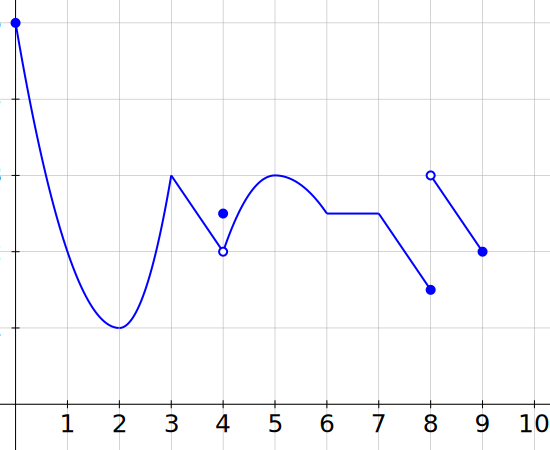
\includegraphics[scale=.42]{G13}
		\end{center}
	\end{frame}
	

	%\begin{frame}[t]
	%	\frametitle{True or False --- Local Extrema}

	%	Let $I$ be an interval. Let $f$ be a function defined on $I$. Let $c\in I$.

	%	Which implications are true?
	%	\begin{enumerate}
	%		\item IF $f$ has local extreme at $c$ , THEN $f$ has an extreme at $c$
	%		\item IF $f$ has an extreme at $c$, THEN $f$ has local extreme at $c$
	%		\item IF $f$ has a local extreme at $c$, THEN $f' (c ) = 0$.
	%		\item IF $f'(c ) = 0$, THEN $f$ has a local extreme at $c$.
	%		\item None of these.
	%	\end{enumerate}

	%\end{frame}

	\begin{frame}[t]
		\frametitle{How many zeroes?}

		Let
		\[
			f(x) = e^{x}- \sin x + x^{2}+ 10x
		\]

		How many zeroes does $f$ have?
	\end{frame}

	\begin{frame}[t]
		\frametitle{The second Theorem of Rolle}

		Complete the statement for this theorem and prove it.

		\vfill

		\begin{block}{Rolle's Theorem 2}
			Let $a<b$. Let $f$ be a function defined on $[a,b]$. \\ IF
			\begin{itemize}
				\item Some conditions on continuity and derivatives

					\emph{[state these conditions precisely]}

				\item $\displaystyle f(a) = f'(a) =0$

				\item $\displaystyle f(b)=0$
			\end{itemize}
			THEN $\displaystyle \exists c \in (a,b)$ such that $\displaystyle f''(c)=0$.
		\end{block}

		\vfill

		\emph{Hint:} Apply the 1st Rolle's Theorem to $f$, then do something else.
	\end{frame}















\begin{frame}
	\frametitle{MAT137 Lecture 28 --- MVT}

	\vfill
	{\bf Before next class:}
		\begin{itemize} \normalsize
			\item {\bf Watch videos  5.10, 5.11, 5.12}
		\end{itemize}
\end{frame}

	\begin{frame}[t]
		\frametitle{True or False---Local Extrema Again}

		Let $I$ be an \textcolor{red}{open} interval. Let $f$ be a \textcolor{red}{differentiable}
		function defined on $I$. Let $c\in I$.

		Which implications are true?
		\begin{enumerate}
			\item IF $f$ has local extreme at $c$ , THEN $f$ has an extreme at $c$
			\item IF $f$ has an extreme at $c$, THEN $f$ has local extreme at $c$
			\item IF $f$ has a local extreme at $c$, THEN $f' (c ) = 0$.
			\item IF $f'(c ) = 0$, THEN $f$ has a local extreme at $c$.
		\end{enumerate}

	\end{frame}

	\begin{frame}[t]
		\frametitle{Proving difficult identities}

		\begin{block}{}
			Prove that, for every $x \geq 0$,
			\[
				2 \arctan \sqrt{x}- \arcsin \frac{x-1}{x+1}= \frac{\pi}{2}
			\]
		\end{block}

		\emph{Hint:} You are trying to prove a function is constant. Use derivatives.
	\end{frame}
	\begin{frame}[t]
		\setsize{12}
		\frametitle{Critique this ``proof"}
		\begin{itemize}
			\item $\displaystyle  \phantom{\rojo{\frac{d}{dx}}} \left[ 2 \arctan
				\sqrt{x} - \arcsin \frac{x-1}{x+1} \right] =
				\phantom{\rojo{\frac{d}{dx}}} \left[ \frac{\pi}{2} \right] $

			\item $\displaystyle  \rojo{\frac{d}{dx}} \left[ 2 \arctan \sqrt{x} -
				\arcsin \frac{x-1}{x+1} \right] = \rojo{\frac{d}{dx}} \left[
				\frac{\pi}{2} \right] $

			\item $\displaystyle \frac{2}{1+ \left( \sqrt{x}\right)^{2}} \cdot \frac{1}{2\sqrt{x}}
				\; - \; \frac{1}{\sqrt{1- \left( \frac{x-1}{x+1}\right)^{2}}} \cdot \frac{(x+1)
				- (x-1)}{(x+1)^{2}} \; = \; 0$

			\item $\displaystyle \frac{1}{(1+ x)\sqrt{x} } \; - \; \frac{1}{ \sqrt{\frac{4x}{(x+1)^{2}}
				}} \cdot \frac{2}{(x+1)^{2}} \; = \; 0$

			\item $\displaystyle 0 = 0$

			\item So $\displaystyle  2 \arctan \sqrt{x} - \arcsin \frac{x-1}{x+1} $ is
				constant.

			\item Evaluate at $x=0$ to find the value of the constant.

			\item $\displaystyle 2 \arctan 0 \; - \; \arcsin (-1) \; = \; 0 - \left( -
				\pi/2 \right) \; = \; \pi/2 $

			\item Therefore, \;
				$\displaystyle 2 \arctan \sqrt{x} - \arcsin \frac{x-1}{x+1} \; = \; \frac{\pi}{2}$
		\end{itemize}
	\end{frame}
	\begin{frame}[t]
		\smallerfont
		\frametitle{Car race - 1}

		A driver competes in a race.

		\medskip
		Use MVT to prove that at some point during the race the instantaneous
		velocity of the driver is exactly equal to the average velocity of the
		driver during the race.
	\end{frame}
	\begin{frame}[t]
		\smallerfont
		\frametitle{Car race - 2}

		Two drivers start a race at the same moment and finish in a tie.

		\medskip
		Can you conclude that there was a time in the race (not counting the starting
		time) when the two drivers had exactly the same speed?
	\end{frame}
	\begin{frame}[t]
		\smallerfont
		\frametitle{Car race - Is this proof correct?}

		\begin{block}{\smallerfont Claim}
			IF two drivers start a race at the same moment and finish in a tie, THEN
			at some point in the race (not counting the starting time) they had
			exactly the same speed.
		\end{block}

		{\bf Proof?}
		\begin{itemize}
			\item Let $f(t)$ and $g(t)$ be the positions of the two cars at time $t$.

			\item Assume the race happens in the interval $[t_{1},t_{2}]$. By
				hypothesis:
				\[
					f(t_{1}) = g(t_{1}), \quad \quad f(t_{2}) = g(t_{2}).
				\]

			\item Using MVT, there exists $c \in (t_{1}, t_{2})$ such that
				\[
					f'(c) = \frac{f(t_{2}) - f(t_{1})}{t_{2}- t_{1}}, \quad g'(c) = \frac{g(t_{2})
					- g(t_{1})}{t_{2}- t_{1}}.
				\]

			\item Then $f'(c) = g'(c)$. \hfill $\square$
		\end{itemize}
	\end{frame}
	\begin{frame}[t]
		\smallerfont
		\frametitle{Car race - resolution}

		Two drivers start a race at the same moment and finish in a tie.

		\medskip
		Prove that at some point during the race (not counting the starting time)
		the two drivers had exactly the same speed.
	\end{frame}











\begin{frame}
	\frametitle{MAT137 Lecture 29 --- Monotonicity}

	\vfill
	{\bf Before next class:}
		\begin{itemize} \normalsize
			\item {\bf Watch videos  6.1, 6.2}
		\end{itemize}
\end{frame}

	\begin{frame}[t]
		\frametitle{Definition of increasing}

		Let $f$ be defined by $f(x)=x^3$.

		Which statements are TRUE?

		\begin{enumerate}
			\item $f$ is increasing on $(0,\infty)$.
			\item $f$ is increasing on $[0,\infty)$.
			\item $f$ is increasing on $(-\infty, 0)$.
			\item $f$ is increasing on $(-\infty, 0]$.
			\item $f$ is increasing on $(-\infty, 0)$ and on $(0,\infty)$.
			\item $f$ is increasing on $(-\infty, 0]$ and on $[0,\infty)$.
			\item $f$ is increasing on $\mathbb R$.
			\item $f$ is increasing on $[1,2]$.
		\end{enumerate}
	\end{frame}

	\begin{frame}[t]
		\frametitle{True or False---Again, Again!}

		Let $I$ be an \textcolor{red}{open} interval. 

		Let $f$ be a
		function defined on $I$. 

		Let $c\in I$.		Which implications are true?
		\begin{enumerate}
			\item IF $f$ is increasing on $I$ , THEN $\forall x\in I$, $f'(x)>0$.
			\item IF $\forall x\in I$, $f'(x)>0$, THEN $f$ is increasing on $I$.
			\item IF $f$ has a local extreme at $c$, THEN $f' (c ) = 0$.
			\item IF $f'(c ) = 0$, THEN $f$ has a local extreme at $c$.
		\end{enumerate}

	\end{frame}

	\begin{frame}[t]
		\frametitle{Preparation}

		\begin{enumerate}
			\item Let $f$ be a function defined on an interval $I$.

				Write the definition of ``$f$ is increasing on $I$''.
				\vfill

			\item Write the statement of the Mean Value Theorem
				\vfill
		\end{enumerate}

	\end{frame}

	\begin{frame}[t]
		\frametitle{Positive derivative implies increasing}

		Use the MVT to prove

		\begin{block}{Theorem}
			Let $a < b$. Let $f$ be a differentiable function on $(a,b)$.
			\begin{itemize}
				\item IF $\forall x \in (a,b), f'(x) >0$,

				\item THEN $f$ is increasing on $(a,b)$.
			\end{itemize}
		\end{block}

		\pause

		\begin{enumerate}
			\item Recall the definition of what you are trying to prove.

			\item {\bf From that definition, figure out the structure of the proof.}

			\item If you have used a theorem, did you verify the hypotheses?

			\item Are there words in your proof, or just equations?
		\end{enumerate}
	\end{frame}
	\begin{frame}[t]
		\frametitle{What is wrong with this proof?}

		\begin{block}{Theorem}
			Let $a < b$. Let $f$ be a differentiable function on $(a,b)$.
			\begin{itemize}
				\item IF $\forall x \in (a,b), f'(x) >0$,

				\item THEN $f$ is increasing on $(a,b)$.
			\end{itemize}
		\end{block}

		\begin{proof}
			\begin{itemize}
				\item From the MVT, $\displaystyle  f'(c) = \frac{f(b) - f(a)}{b-a} $

				\item We know $\displaystyle b-a>0$ and $\displaystyle f'(c)>0$

				\item Therefore $\displaystyle f(b) - f(a)>0$. \quad Thus
					$\displaystyle f(b) > f(a)$.

				\item $f$ is increasing.
			\end{itemize}
		\end{proof}
	\end{frame}
	\begin{frame}[t]
		\frametitle{Inequalities}

		Prove that, for every $x \in \mathbb{R}$
		\[
			e^{x}\geq 1 + x
		\]

		\medskip
		\emph{Hint:} Where is the function $\displaystyle f(x) =e^x - 1-x$ increasing
		or decreasing? What is its minimum?
	\end{frame}











%	%-----------------------------
%	\begin{frame}[t]
%		\frametitle{What can you conclude?}
%
%		We know the following about the function $f$.
%		\begin{itemize}
%			\item $f$ has domain $\mathbb{R}$.
%
%			\item $f$ is continuous
%
%			\item $f(0)=0$
%
%			\item For every $x \in \mathbb{R}$, $f(x) \geq x$.
%		\end{itemize}
%		\begin{block}{}
%			What can you conclude about $f'(0)$? Prove it.
%		\end{block}
%
%		\vfill
%
%		\emph{Hint:} Sketch the graph of $f$. Looking at the graph, make a
%		conjecture. \\ To prove it, imitate the proof of the Local EVT from Video
%		5.3.
%	\end{frame}
%
%	%-----------------------------
%	%-----------------------------
%	%-----------------------------
%	%-----------------------------
%	\begin{frame}[t]
%		\frametitle{Zeroes of the derivative}
%
%		Sketch the graph of a function $f$ that is differentiable on $\mathbb{R}$
%		and such that
%
%		\medskip
%		\begin{enumerate}
%			\item $f$ has exactly 3 zeroes and $f'$ has exactly 2 zeroes.
%
%			\item $f$ has exactly 3 zeroes and $f'$ has exactly 3 zeroes.
%
%			\item $f$ has exactly 3 zeroes and $f'$ has exactly 1 zero.
%
%			\item $f$ has exactly 3 zeroes and $f'$ has infinitely many zeroes.
%		\end{enumerate}
%	\end{frame}
%	%-----------------------------
%	\begin{frame}[t]
%		\frametitle{Zeroes of a polynomial}
%
%		You probably learned in high school that a polynomial of degree $n$ has at
%		most $n$ real zeroes. Now you can prove it!
%
%		\medskip
%		\emph{Hint:} Use induction. If you are having trouble, try the case $n=3$
%		first.
%	\end{frame}
%	%-----------------------------
%	%-----------------------------
%	\begin{frame}[t]
%		\frametitle{The $N$-th Theorem of Rolle}
%
%		Complete the statement for this theorem and prove it.
%
%		\medskip
%		\begin{block}{Rolle's Theorem $N$}
%			Let $N$ be a positive integer. \\ Let $a<b$. Let $f$ be a function defined
%			on $[a,b]$. \\ IF
%			\begin{itemize}
%				\item (Some conditions on continuity and derivatives)
%
%				\item (Some conditions at $a$)
%
%				\item $\displaystyle f(b)=0$
%			\end{itemize}
%			THEN $\displaystyle \exists c \in (a,b)$ such that
%			$\displaystyle f^{(N)}(c)=0$.
%		\end{block}
%	\end{frame}
%
%	%-----------------------------
%
%	\begin{frame}[t]
%		\smallerfont
%		\frametitle{A new theorem}
%
%		We want to prove this theorem:
%		\begin{block}{\smallerfont Theorem 1}
%			Let $f$ be a differentiable function on an open interval $I$. \\ IF
%			$\displaystyle \forall x \in I, f'(x) \neq 0$ \\ THEN $f$ is one-to-one on
%			$I$.
%		\end{block}
%
%		\vfill
%		\pause
%
%		\begin{enumerate}
%			\item Transform \quad $\displaystyle [P \implies Q]$ \quad into \quad $\displaystyle
%				[(\mbox{not } Q) \implies (\mbox{not } P)]$. \\ You get an equivalent
%				Theorem (call it ``Theorem 2"). \\ We are going to prove Theorem 2
%				instead.
%
%			\item Write the definition of ``$f$ is not one-to-one on $I$". You will need
%				it.
%
%			\item Recall the statement of Rolle's Theorem. You will need it.
%
%			\item Do some rough work if needed.
%
%			\item Write a complete proof for Theorem 2.
%		\end{enumerate}
%	\end{frame}
%
%	%-----------------------------
%	\begin{frame}[t]
%		\frametitle{A variant}
%
%		Complete this variation on Theorem 2. \\ Use the weakest conditions you can
%		to make it true.
%
%		\medskip
%		\begin{block}{Theorem 3}
%			Let $a<b$. Let $f$ be a function defined on $[a,b]$. \\ IF
%			\begin{itemize}
%				\item (Some conditions on continuity and differentiability)
%
%				\item $f$ is not one-to-one on $[a,b]$
%			\end{itemize}
%			THEN $\displaystyle \exists c \in (a,b)$ such that $f'(c)=0$.
%		\end{block}
%	\end{frame}
%
%	%-----------------------------
%	\begin{frame}
%		\frametitle{Why the three hypotheses are necessary}
%
%		You have proven
%
%		\begin{block}{Theorem 3}
%			Let $a<b$. Let $f$ be a function defined on $[a,b]$. \\ IF
%			\begin{enumerate}
%				\item $f$ is continuous on $[a,b]$
%
%				\item $f$ is differentiable on $(a,b)$
%
%				\item $f$ is not one-to-one on $[a,b]$
%			\end{enumerate}
%			THEN $\displaystyle \exists c \in (a,b)$ such that $f'(c)=0$.
%		\end{block}
%
%		\vfill
%
%		Give three examples to justify that each of the three hypotheses are necessary
%		for the theorem to be true. (Graphs of the examples are enough).
%	\end{frame}
%	%-----------------------------
%	\begin{frame}[t]
%		\frametitle{MVT -- True or False?}
%
%		\begin{block}{True or False}
%			Consider $f(x) = |x|$ on the interval $[-\frac{1}{2}, 2]$.
%
%			There exists $c$ in $(-\frac{1}{2},2)$ such that
%			\[
%				f'(c) = \frac{f(2) - f(-\frac{1}{2})}{2-(-\frac{1}{2})}
%			\]
%		\end{block}
%		%This is a quick warm up question to make sure that students watched the video and understand that we need to check that all the hypotheses are satisfied before using the theorem.
%	\end{frame}
%
%	%-----------------------------
%
%	%-----------------------------
%	%-----------------------------
%
%	%-----------------------------
%
%	%-----------------------------
%	\begin{frame}[t]
%		\smallerfont
%		\frametitle{Speeding ticket!}
%
%		On a toll road Barney takes a time stamped toll-card from the starting booth
%		and drives directly to the end of the toll section. \\
%		\vspace{.2cm}
%
%		After paying the required toll, Barney is surprised to receive a speeding ticket
%		along with the toll receipt. \\
%		\vspace{.2cm}
%
%		Which of the following are true?
%		\vspace{.2cm}
%		\begin{enumerate}
%			\item The booth attendant does not have enough information to prove that Barney
%				was speeding.
%
%			\item The booth attendant can prove that Barney was speeding during his trip.
%
%			\item Barney's ticket is for a lower speed than his actual maximum speed.
%		\end{enumerate}
%	\end{frame}
%	%-----------------------------
%	%------------------------------------
%	%-----------------------------
%	\begin{frame}[t]
%		\frametitle{Warm up}
%
%		\begin{enumerate}
%			\item Let $f$ be a function defined on an interval $I$.
%
%				Write the definition of ``$f$ is increasing on $I$".
%
%				\medskip
%
%
%			\item Write the statement of the Mean Value Theorem.
%		\end{enumerate}
%	\end{frame}
%	%-----------------------------
%
%
%	%-----------------------------
%	%-----------------------------
%	\begin{frame}[t]
%		\frametitle{Your first integration}
%
%		Find all functions $f$ such that, for all $\displaystyle x \in \mathbb{R}$:
%		$\displaystyle f''(x) = x + \sin x$.
%	\end{frame}
%
%	%-----------------------------
%
%	\begin{frame}
%		\frametitle{Intervals of monotonicity}
%
%		Let $\displaystyle  g(x) = x^3(x^2-4)^{1/3}. $
%
%		\medskip
%		Find out on which intervals this function is increasing or decreasing.
%
%		Using that information, sketch its graph.
%
%		\medskip
%		To save time, here is the first derivative:
%		\[
%			g'(x) = \frac{x^{2}(11x^{2}-36)}{3(x^{2}-4)^{2/3}}
%		\]
%	\end{frame}
%
%	%-----------------------------
%	\begin{frame}[t]
%		\smallerfont
%		\frametitle{True or False -- Monotonicity and local extrema}
%
%		Let $I$ be an interval. Let $f$ be a function defined on $I$. Let $c \in I$.
%		Which implications are true?
%
%		\medskip
%		\begin{enumerate}
%			\item IF \rojo{$f$ is increasing on $I$}, \quad THEN \azul{$\forall x \in I$, $f'(x) >0$}.
%
%			\item IF \azul{$\forall x \in I$, $f'(x) >0$}, \quad THEN \rojo{$f$ is increasing on $I$}.
%
%				\medskip
%
%
%			\item IF \rosa{$f$ has a local extremum at $c$}, \quad THEN \naranja{$f'(c)=0$}.
%
%			\item IF \naranja{$f'(c)=0$}, \quad THEN \rosa{$f$ has a local extremum at $c$}.
%
%				\medskip
%
%
%			\item IF \rosa{$f$ has local extremum at $c$}, \; THEN \verde{$f$ has an extremum at $c$}
%
%			\item IF \verde{$f$ has an extremum at $c$}, \; THEN \rosa{$f$ has local extremum at $c$}
%		\end{enumerate}
%	\end{frame}
%
%	%-----------------------------
%
%	%-----------------------------
%	\begin{frame}[t]
%		\frametitle{Backwards graphing}
%
%		Below is the graph of a polynomial $P$. Notice that it is not at scale. The
%		coordinates in the graph are $a=24$, $b=25$, and $c=1$. Find the equation of
%		$P$.
%
%		\begin{center}
%			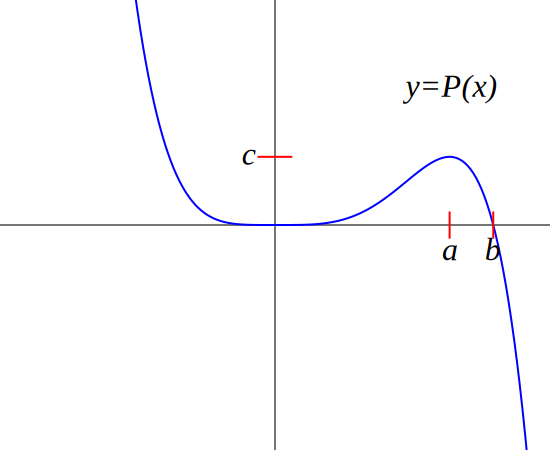
\includegraphics[scale=.38]{G18}
%		\end{center}
%	\end{frame}
%
%	%-----------------------------
%	\begin{frame}[t]
%		\frametitle{A sneaky function}
%
%		Construct a function $f$ satisfying all the following properties:
%
%		\medskip
%		\begin{itemize}
%			\item Domain $\displaystyle f = \mathbb{R}$
%
%			\item $f$ is continuous
%
%			\item $f'(0)=0$
%
%			\item $f$ does not have a local extremum at $0$.
%
%			\item There isn't an interval centered at $0$ on which $f$ is increasing.
%
%			\item There isn't an interval centered at $0$ on which $f$ is decreasing.
%		\end{itemize}
%	\end{frame}

	%------------------------------
	%-----------------------------
\end{document}
%-----------------------------
%-----------------------------
